\subsection{Topological codes}
Previous research in computer science 
provides a toolset for generating valid codes
from existing encoding schemes. 
Hypergraph product codes, introduced by Tillich and Z\'emor,
of two 
existing codes will always remain a valid detection code.

The parity check matrix $H$ of a hypergraph product code is generated
by two m by n parity check matrices of valid codes in the following
way:
\begin{equation}
	H = \left(\begin{array}{cc}
		\left(M_{pc1} \otimes \mathbb{I}_{n_2}| 
        \mathbb{I}_{m_1} \otimes M_{pc2}^T \right) & 0 \\
		0 & \left(\mathbb{I}_{n_1}\otimes 
        M_{pc2} | M_{pc1}^T \otimes \mathbb{I}_{m_2}\right)\\
	\end{array}\right)
\end{equation}

\subsubsection{Surface code}
We can therefore form a hypergraph product code of two repetition
codes to
obtain the [[$d^2$,1,d]] ``Surface-Code'' which can detect up
to d of $both$ X and Z errors, and 
therefore any error happening \cite{joschka}.
We can draw this code as a graph, whereby the code's stabilizers
are understood as an adjacency Matrix of data to ancilla qubits.
Like the repetition code, the Surface code is a code that is regular until
its boundary nodes. 
The logical operators on the surface code are lines that go from one 
boundary to another that lies across, as this triggers every ancilla along
the way twice, thus nonce, and therefore takes the message back to the
codespace.

\begin{figure}[h!]
	\begin{center}
	\captionsetup{justification=centering,margin=2cm}
	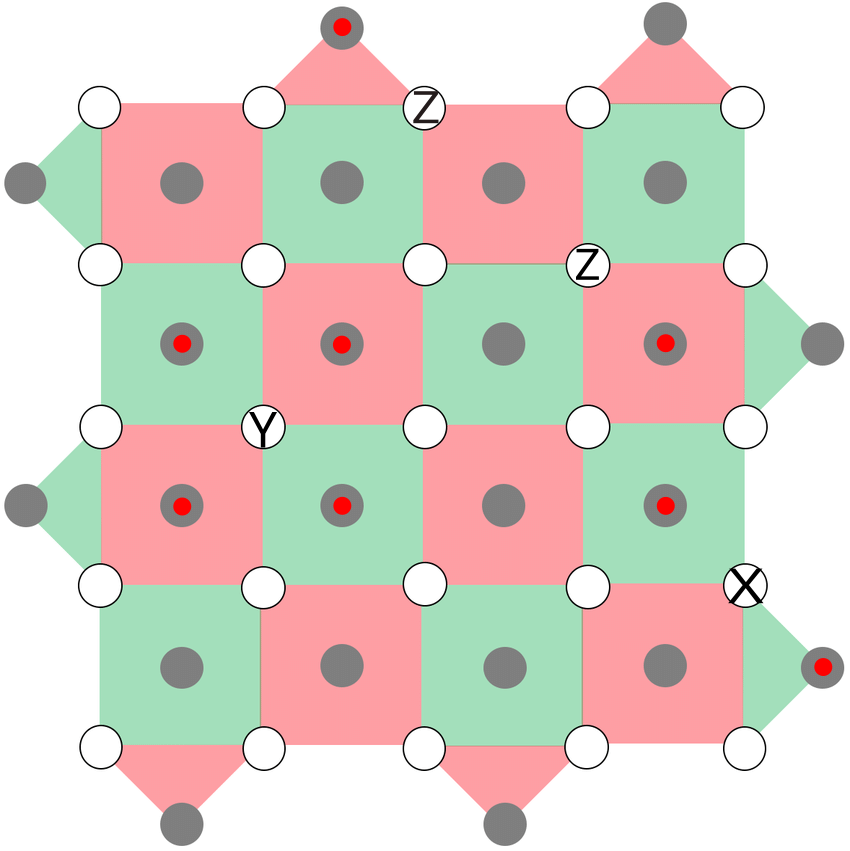
\includegraphics[scale=0.35]{./img/figures/d5surfaceCode.png}\\
	\caption{Distance 5 Surface code with data qubits in white and 
    ancilla qubits in grey. Green Faces represent Z stabilizers
    and Red faces represent X stabilizers.
    Errors on data qubits are marked
    by respective Pauli names and violated stabilizers are marked in red.}
	\label{fig: surface_code}
	\end{center}
\end{figure}


INCLUDE LOGICAL OPERATORS
\newpage

\subsubsection{Toric code}
Similarly, a hypergraph product code of two ring codes can be 
generated. We call this code the "Toric code".\\
\begin{figure}[h!]
	\begin{center}
	\captionsetup{justification=centering,margin=2cm}
	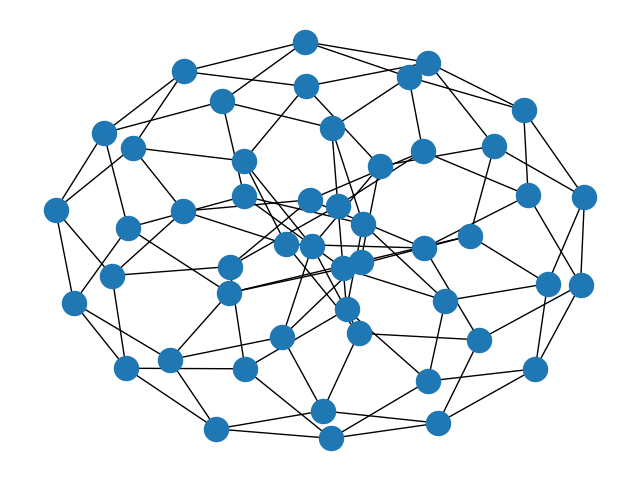
\includegraphics[scale=0.4]{./img/figures/toric_5_graph.png}\\
	\caption{Graph for [[49,1,7]] toric code}
        
	\label{fig: toric_graph}
	\end{center}
\end{figure}
Notably, this resembles a donut, or torus.
The logical operators on the toric code are loops, so a circle of 
'errors' on nodes is a logical X operator, and a circle of 'errors'
on faces is a logical Z operator.
\newpage

\subsubsection{Color code}
The color code's parity-check-matrix's 
rows are both the code's X stabilizers and Z stabilizers.
Any three-colorable and three-valent graph represents a valid color code.
On the color code, an error is bounded by syndromic faces of all colors.
The simplest color code is the [[7,1,3]] Steane code \cite{steane}. 
\\
\begin{figure}[h!]
	\begin{center}
	\captionsetup{justification=centering,margin=2cm}
	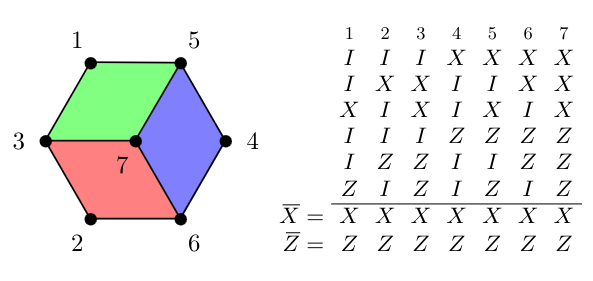
\includegraphics[scale=0.6]{./img/figures/steane.png}\\
	\caption{Graph for the [[7,1,3]] color code, also known as the
    Steane code , and its stabilizers. 
    Figure from \cite{steane}.}
        
	\label{fig: color_graph}
	\end{center}
\end{figure}
% habe ich von erster google bildsuchen seite
